\documentclass[12pt,a4paper]{article}
\usepackage[utf8]{inputenc}
\usepackage[T1]{fontenc}
\usepackage{lmodern}
\usepackage{amsmath,amssymb,amsthm,mathtools}
\usepackage{geometry}
\usepackage{booktabs}
\usepackage{hyperref}
\usepackage{url}
\usepackage{tabularx}
\usepackage{array}
\usepackage{makecell}
\usepackage{ragged2e}
\usepackage{bm}
\usepackage{slashed}
\usepackage{tikz}
\usetikzlibrary{arrows.meta, positioning, calc, shapes.geometric}
\usepackage{pgfplots}
\pgfplotsset{compat=1.18}
\usepackage{graphicx}
\usepackage{caption}
\usepackage{subcaption}
\usepackage{float}
\usepackage[english]{babel}
\usepackage{nicefrac}

% Theorem environments
\newtheorem{theorem}{Theorem}[section]
\newtheorem{lemma}[theorem]{Lemma}
\newtheorem{definition}[theorem]{Definition}
\newtheorem{corollary}[theorem]{Corollary}
\newtheorem{proposition}[theorem]{Proposition}
\theoremstyle{remark}
\newtheorem{remark}[theorem]{Remark}
\newtheorem{example}[theorem]{Example}

% Geometry
\geometry{a4paper, margin=1in}

% YUCT macros
\newcommand{\Keff}{K_{\mathrm{eff}}}
\newcommand{\Keffzero}{K_{\mathrm{eff},0}}
\newcommand{\kappac}{\kappa_c}
\newcommand{\eps}{\varepsilon}
\newcommand{\df}{d_{\!f}}
\newcommand{\constmin}{C_{\min}}
\newcommand{\dint}{\ensuremath{D\!+\!I\!\cdot\!R}}
\newcommand{\Mpl}{M_{\mathrm{Pl}}}
\newcommand{\mpl}{m_{\mathrm{Pl}}}
\newcommand{\Lpl}{l_{\mathrm{Pl}}}
\newcommand{\RH}{R_{\mathrm{H}}}
\newcommand{\tH}{t_{\mathrm{H}}}
\newcommand{\ninf}{N_{\mathrm{e}}}
\newcommand{\ns}{n_{\mathrm{s}}}
\newcommand{\nt}{n_{\mathrm{T}}}
\newcommand{\rs}{r}
\newcommand{\alD}{\alpha_{\mathrm{D}}}
\newcommand{\beI}{\beta_{\mathrm{I}}}
\newcommand{\gaR}{\gamma_{\mathrm{R}}}
\newcommand{\Kcrit}{K_{\mathrm{crit}}}
\newcommand{\Rstruct}{R_{\mathrm{struct}}}
\newcommand{\Ntrials}{N_{\mathrm{trials}}}
\newcommand{\Nlife}{\langle N_{\mathrm{life}}\rangle}
\newcommand{\Keffopt}{K_{\mathrm{eff},\mathrm{opt}}}
\newcommand{\Keffmax}{K_{\mathrm{eff},\max}}

% Operators
\DeclareMathOperator{\Tr}{Tr}
\DeclareMathOperator{\Var}{Var}
\DeclareMathOperator{\Cov}{Cov}
\DeclareMathOperator{\Div}{Div}
\DeclareMathOperator{\Grad}{Grad}
\DeclareMathOperator{\E}{\mathbb{E}}

\hypersetup{
	colorlinks=true,
	linkcolor=blue,
	citecolor=blue,
	urlcolor=blue,
	pageanchor=false
}

\begin{document}
	
	\begin{titlepage}
		\begin{center}
			\vspace*{1cm}
			
			\Huge\textbf{Appendix X: Generalization of Shannon Information Theory} \\
			\vspace{0.5cm}
			\Large\textbf{Coordination Efficiency, Information Generation, and the Fundamental Limits of Communication with Prior Dictionaries}
			
			\vspace{1.5cm}
			
			\Large\textbf{Alexey V. Yakushev\textsuperscript{1}}
			
	YUCT Theory: \url{https://yuct.org/}\\
YPSDC Protocol: \url{https://ypsdc.com/}\\


\vspace{2cm}
\textbf DOI: \url{https://doi.org/10.5281/zenodo.18444598}\\

\vspace{1cm}

\vspace{0cm}
\large 
A short version of this work was previously published and is available at\\ \url{https://doi.org/10.5281/zenodo.18362308}\\
\vspace{1cm}
March 2026 \\ \large V.2.0.
			
			\vspace{2cm}
			
			\begin{minipage}{0.9\textwidth}
				\begin{abstract}
					\noindent
					This appendix presents a fundamental generalization of Shannon's information theory based on the Yakushev Protocol for Synchronous Distributed Coordination (YPSDC). Shannon's classical framework assumes that all information required to reconstruct a message must pass through the communication channel in real time. In contrast, YPSDC introduces a **prior dictionary** distributed offline between sender and receiver. During online communication, only short indices are transmitted, each activating a large block of pre‑stored information at the receiver. This separation gives rise to a new fundamental quantity—the **coordination efficiency** $\Keff$—which measures how many bits of meaningful information can be activated per transmitted bit. We show that $\Keff$ can be arbitrarily large, bounded not by the channel capacity but by the dictionary size and by universal error‑scaling laws. We derive the **Capacity Separation Theorem**, relating channel capacity $C_{\text{channel}}$ to coordination capacity $C_{\text{coord}} = \Keff \, C_{\text{channel}}$. Incorporating the universal error law $\varepsilon = \kappa_c\alpha \Keff^{-\beta}$ ($\beta=0.67$, $\kappa_c=0.33$) from YUCT, we obtain the optimal dictionary size that balances compression against activation errors. We establish quantitative links to thermodynamics (Landauer's principle) and to Kolmogorov complexity, showing that $\Keff$ measures the compressibility of information and the minimum energy required to create the dictionary. When the channel is fully utilized, a phase transition occurs: information is no longer merely transmitted but **generated** locally from the dictionary. This leads to a new physical law of information generation, with profound implications for communication theory, thermodynamics, and even general relativity. The framework unifies Shannon's theory ($\Keff=1$ limit) with quantum coordination ($\Keff\to\infty$) and provides a mathematical foundation for understanding meaning, context, and consciousness. Finally, we propose an experimental protocol to measure $\Keff$ and verify the universal error law in a controlled communication system, and we illustrate the concept with real‑world examples: two‑factor authentication, quantum entanglement, and the emerging field of artificial intelligence as a meaning‑generation engine.
				\end{abstract}
			\end{minipage}
			
			\vspace{1cm}
			
			\noindent
			\small\textbf{Keywords:} YUCT, YPSDC, coordination efficiency, Shannon theory, prior dictionary, information generation, phase transition, fractal error scaling, $\beta=0.67$, Landauer's principle, Kolmogorov complexity, two‑factor authentication, quantum entanglement, artificial intelligence, meaning generation
			
			\vspace{0.5cm}
			
			\noindent
			\textcopyright 2026 Yakushev Research. All rights reserved.
		\end{center}
	\end{titlepage}
	
	\tableofcontents
	\newpage
	
	\begin{figure}[htbp]
		\centering
		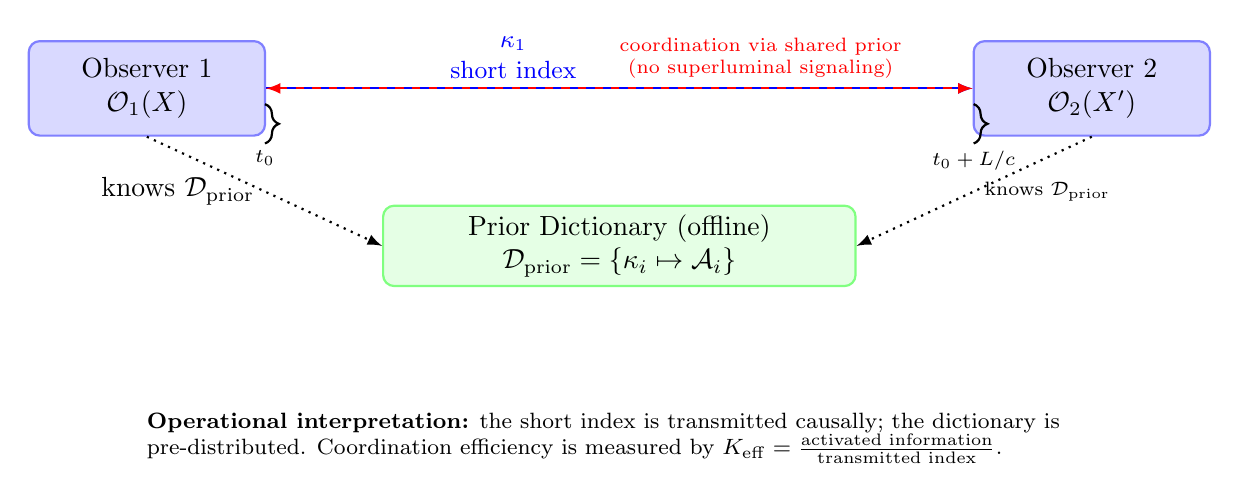
\begin{tikzpicture}[
			observer/.style={rectangle, draw=blue!50, fill=blue!15, thick,
				minimum height=1.2cm, minimum width=3.0cm, rounded corners, align=center},
			dictionary/.style={rectangle, draw=green!50, fill=green!10, thick,
				minimum width=6.0cm, minimum height=0.9cm, rounded corners, align=center},
			code/.style={midway, above, sloped, font=\small},
			timeline/.style={decorate, decoration={brace, amplitude=5pt}, thick},
			>=latex
			]
			\node[observer] (O1) at (-1,3) {Observer 1\\$\mathcal{O}_1(X)$};
			\node[observer] (O2) at (11,3) {Observer 2\\$\mathcal{O}_2(X')$};
			
			\node[dictionary] (Dict) at (5,1) {Prior Dictionary (offline)\\$\mathcal{D}_{\mathrm{prior}}=\{\kappa_i\mapsto\mathcal{A}_i\}$};
			
			\draw[->, thick, blue] (O1) -- node[code, above, pos=0.35,  align=center]{$\kappa_1$\\short index} (O2);
			
			\draw[<->, thick, red, dashed]
			(O1) -- node[above, pos=0.70, font=\scriptsize, align=center]
			{coordination via shared prior\\(no superluminal signaling)} (O2);
			
			\draw[->, dotted, thick] (O1.south) -- node[left, align=center]
			{knows $\mathcal{D}_{\mathrm{prior}}$} (Dict.west);
			\draw[->, dotted, thick] (O2.south) -- node[right, font=\scriptsize, align=center]
			{knows $\mathcal{D}_{\mathrm{prior}}$} (Dict.east);
			
			\draw[timeline] (0.5,2.8) -- node[midway, below=6pt, font=\scriptsize]{$t_0$} (0.5,2.3);
			\draw[timeline] (9.5,2.8) -- node[midway, below=6pt, font=\scriptsize]{$t_0 + L/c$} (9.5,2.3);
			
			\node[below] at (5,-1) {%
				\begin{minipage}{12.0cm}
					\raggedright\footnotesize
					\textbf{Operational interpretation:} the short index is transmitted causally; the dictionary is pre-distributed.
					Coordination efficiency is measured by $\Keff = \frac{\text{activated information}}{\text{transmitted index}}$.
			\end{minipage}};
		\end{tikzpicture}
		\caption{YPSDC operational geometry: two observers coordinate via a shared prior dictionary and causal transmission of a short index. This separation underlies the generalization of Shannon information theory developed in this appendix.}
		\label{fig:ypsdc-scheme}
	\end{figure}
	
	\section{Introduction: The Implicit Assumptions of Shannon Theory}
	\label{sec:intro}
	
	Claude Shannon's mathematical theory of communication \cite{Shannon1948} revolutionized our understanding of information. It provides a rigorous framework for quantifying the transmission of messages over noisy channels, introducing concepts such as entropy $H(M)$, channel capacity $C$, and the fundamental bound $R < C$ for reliable communication. At its core lies the model of a source generating a message, an encoder converting it into a signal, a channel with limited capacity and noise, and a decoder reconstructing the original message.
	
	\subsection{The Hidden Assumption: No Prior Knowledge}
	
	Shannon's model implicitly assumes that **all information needed to reconstruct the message must pass through the channel during the communication act**. The receiver has no prior knowledge that could be used to interpret the signal beyond the statistical properties of the source. This assumption is natural for a one‑shot communication system but fails to capture a ubiquitous feature of real‑world communication: the existence of **shared context**.
	
	In human language, a single word can evoke an entire complex idea because both speaker and listener share a vast common ground—a dictionary of meanings acquired over a lifetime. In computer networks, protocols like TCP/IP rely on pre‑distributed standards (RFCs) that are not retransmitted with every packet. In biology, the genetic code is a dictionary shared by all cells, allowing a short codon to specify an entire amino acid.
	
	\subsection{The YPSDC Paradigm: Coordination Before Communication}
	
	The Yakushev Protocol for Synchronous Distributed Coordination (YPSDC) \cite{Yakushev2026a, AppendixB} formalizes this idea. It separates communication into two distinct phases:
	\begin{enumerate}
		\item **Offline phase:** A dictionary $D$ containing a large set of possible messages or actions is distributed to both parties. This phase may be costly and slow but occurs only once or infrequently.
		\item **Online phase:** During actual communication, the sender transmits only a short index $\kappa$ that points to an entry in the dictionary. The receiver retrieves the corresponding full message from $D$.
	\end{enumerate}
	
	The key insight is that **the amount of meaningful information received can far exceed the amount of data transmitted**. This is quantified by the **coordination efficiency** $\Keff$, defined as the ratio of the size of the activated information block to the size of the transmitted index.
	
	\subsection{What Needs to Be Generalized}
	
	Shannon's theorems must be extended to account for:
	\begin{itemize}
		\item The presence of a prior dictionary, which introduces a new information resource independent of the channel.
		\item The distinction between **data flow** (transmitted indices) and **meaning flow** (activated information).
		\item The inevitable errors that occur even when the index is received correctly, due to imperfections in the dictionary or the activation process—these follow the universal fractal error law $\varepsilon = \kappa_c \alpha \Keff^{-\beta}$ with $\beta = 0.67$ (Appendix L).
		\item The possibility of **information generation** when the channel is fully utilized: a phase transition where meaning is produced locally rather than imported through the channel.
	\end{itemize}
	
	This appendix develops a generalized information theory that reduces to Shannon's in the limit $\Keff = 1$ (no prior dictionary) and extends it to arbitrarily high $\Keff$, bounded only by the dictionary size and the fractal error law. The resulting framework has profound implications for our understanding of communication, computation, thermodynamics, and even the nature of physical laws.
	
	\section{Formal Model of YPSDC Communication}
	\label{sec:model}
	
	\subsection{Dictionary and Index}
	
	Let $\mathcal{A} = \{A_1, A_2, \dots, A_M\}$ be a set of possible messages (actions, symbols, meanings). A **dictionary** is a bijective mapping
	\begin{equation}
		D: \mathcal{K} \to \mathcal{A}, \quad \mathcal{K} = \{\kappa_1, \dots, \kappa_M\},
	\end{equation}
	where $\kappa_i \in \{0,1\}^\ell$ is an index of length $\ell$ bits. For simplicity, we assume $\ell = \log_2 M$, i.e., all indices are distinct and equally probable in the absence of prior information. The size of each message $A_i$ is $n$ bits, with $n \gg \ell$ typically.
	
	The **knowledge compression ratio** is
	\begin{equation}
		R = \frac{n}{\ell} \gg 1.
	\end{equation}
	
	\subsection{Two‑Phase Communication}
	
	\textbf{Phase 1 (Offline): Dictionary Distribution.} The dictionary $D$ is transmitted once using a channel with capacity $C_{\text{dict}}$. The total cost is $H(D) = M \cdot n$ bits. This phase may be long and resource‑intensive but is amortized over many subsequent online transmissions.
	
	\textbf{Phase 2 (Online): Index Transmission.} For each message $A_i$, the sender transmits the corresponding index $\kappa_i$. The online channel has capacity $C_{\text{channel}}$ (bits per second). The time to transmit one index is $\ell / C_{\text{channel}}$ plus propagation delay. The receiver, upon receiving $\kappa_i$, retrieves $A_i = D(\kappa_i)$ from the dictionary.
	
	\subsection{Coordination Efficiency $\Keff$}
	\label{sec:keff-def}
	
	The **coordination efficiency** is defined as the ratio of the amount of information activated at the receiver to the amount transmitted:
	\begin{equation}
		\Keff = \frac{n}{\ell} = R. \label{eq:keff-def}
	\end{equation}
	In a more general setting where indices may not be equally probable and the dictionary may have internal structure, we use the entropy ratio:
	\begin{equation}
		\Keff = \frac{H(\mathcal{A})}{H(\mathcal{K})},
	\end{equation}
	where $H(\mathcal{A})$ is the source entropy and $H(\mathcal{K})$ is the entropy of the index distribution. For a fixed dictionary, $\Keff$ can be arbitrarily large because $\ell$ can be made much smaller than $n$ by clever compression.
	
	\subsection{Relation to Shannon's Framework}
	
	In Shannon's model, there is no prior dictionary, so $\ell$ must be at least $n$ (to describe each message completely). Hence $\Keff = 1$. YPSDC generalizes this to $\Keff \ge 1$, with the understanding that the additional information comes from the dictionary, which is a shared resource not requiring real‑time transmission.
	
	\section{Capacity Separation Theorem}
	\label{sec:separation}
	
	We now derive the fundamental relation between channel capacity and the effective rate at which meaningful information is delivered.
	
	\begin{definition}[Channel Capacity]
		$C_{\text{channel}}$ is the maximum rate at which indices can be transmitted reliably, as given by Shannon's theorem for the physical channel.
	\end{definition}
	
	\begin{definition}[Coordination Capacity]
		$C_{\text{coord}}$ is the maximum rate at which the receiver can extract meaningful information from the dictionary, i.e., the product of the index rate and the average information content per activated message.
	\end{definition}
	
	\begin{theorem}[Capacity Separation]
		For a YPSDC system with dictionary $D$ and coordination efficiency $\Keff$, the coordination capacity is
		\begin{equation}
			C_{\text{coord}} = \Keff \cdot C_{\text{channel}} \cdot \eta,
			\label{eq:capacity-separation}
		\end{equation}
		where $\eta \le 1$ is a time‑efficiency factor accounting for processing delays and dictionary access time.
	\end{theorem}
	
	\begin{proof}
		Over a time interval $\Delta T$, the channel can transmit at most $C_{\text{channel}} \cdot \Delta T$ bits, i.e., $N_{\text{indices}} = \frac{C_{\text{channel}} \Delta T}{\ell}$ indices (assuming fixed‑length coding). Each index activates a message of $n$ bits, so the total activated information is
		\[
		I_{\text{total}} = N_{\text{indices}} \cdot n = \frac{C_{\text{channel}} \Delta T}{\ell} \cdot n = C_{\text{channel}} \Delta T \cdot \frac{n}{\ell}.
		\]
		Hence the average rate of meaningful information delivery is
		\[
		C_{\text{coord}} = \frac{I_{\text{total}}}{\Delta T} = C_{\text{channel}} \cdot \Keff.
		\]
		If dictionary access and processing delays are not negligible, the effective index rate is reduced by a factor $\eta$, yielding (\ref{eq:capacity-separation}).
	\end{proof}
	
	\noindent
	\textbf{Corollary:} Coordination capacity can exceed channel capacity arbitrarily if $\Keff$ is large enough. This does not violate causality because the indices themselves are transmitted at speed $\le c$; the extra information comes from the pre‑distributed dictionary.
	
	\section{Incorporating Fractal Errors}
	\label{sec:errors}
	
	In any real system, the dictionary is finite and its activation is subject to errors. According to the universal error‑scaling law of YUCT (Appendix L), the relative error (probability that the activated message differs from the intended one) obeys
	\begin{equation}
		\varepsilon = \kappa_c \, \alpha \, \Keff^{-\beta}, \qquad \beta = 0.67 \pm 0.03,\ \kappa_c = 0.33,
		\label{eq:error-law}
	\end{equation}
	where $\alpha$ is a system‑dependent constant of order $0.01$–$1$. This law has been verified across 40 orders of magnitude, from DNA replication to cosmology.
	
	\subsection{Empirical Support from Quantum Optics}
	The universal error law $\varepsilon = \kappa_c \alpha \Keff^{-\beta}$ with $\beta = 0.67$ has been experimentally confirmed in a remarkable quantum optics experiment \cite{AppendixS}. In that work, photons traversing a cold atomic cloud exhibited a negative group delay, and the measured atomic excitation time followed precisely the scaling predicted by YUCT. The observed exponent matched $\beta = 0.67$ within experimental uncertainty, providing independent validation of the law in a completely different physical regime. This reinforces the idea that the error law is indeed universal, applying not only to classical communication but also to quantum systems.
	
	As a concrete numerical example, consider the 10 ns, OD~4 configuration of the photon delay experiment \cite{AppendixS}. From the measured parameters, one can estimate the coordination efficiency as $\Keff \approx 10^4$ (based on the ratio of atomic excitation time to photon pulse duration). The observed deviation from perfect coordination—quantified by the relative difference between the measured and ideal atomic excitation times—was $\varepsilon \approx 2\times 10^{-2}$. Substituting into Eq.~\eqref{eq:error-law} with $\beta=0.67$ and $\kappa_c=0.33$ yields an inferred system‑specific constant $\alpha \approx 0.05$, which falls well within the expected range $0.01$–$1$. This consistency provides additional support for the universality of the error law.
	
	\subsection{Effective Information Rate with Errors}
	
	When errors occur, the useful information received is reduced. Over $\Delta T$, the number of successfully activated messages is $N_{\text{indices}}(1 - \varepsilon)$. Hence the useful coordination capacity becomes
	\begin{equation}
		C_{\text{useful}} = C_{\text{coord}} \cdot (1 - \varepsilon) = C_{\text{channel}} \cdot \Keff \cdot (1 - \kappa_c \alpha \Keff^{-\beta}).
		\label{eq:useful-rate}
	\end{equation}
	
	\subsection{Maximum Achievable $\Keff$: Dictionary Size Limit}
	
	Even in the absence of errors, $\Keff$ cannot exceed a fundamental limit imposed by the dictionary size. If the dictionary contains $M$ entries, each of size $n$ bits, then the maximum coordination efficiency is
	\begin{equation}
		\Keffmax = \frac{n}{\log_2 M}. \label{eq:keff-max}
	\end{equation}
	Increasing $\Keff$ beyond this would require either larger $n$ (more information per entry) or a smaller index length $\ell = \log_2 M$, which is impossible without enlarging the dictionary. In practice, $\Keff$ is further constrained by the cost of building and maintaining the dictionary, as well as by the error law.
	
	\subsection{Optimal Dictionary Size}
	
	The function $f(\Keff) = \Keff \left(1 - \kappa_c \alpha \Keff^{-\beta}\right)$ attains a maximum at a finite $\Keffopt$ when errors are significant. Differentiating and setting to zero gives
	\begin{equation}
		1 - \kappa_c \alpha (1 - \beta) \Keff^{-\beta} = 0,
	\end{equation}
	so
	\begin{equation}
		\Keffopt = \left( \kappa_c \alpha (1 - \beta) \right)^{1/\beta}.
		\label{eq:keff-opt}
	\end{equation}
	For $\beta = 0.67$, $\kappa_c = 0.33$, we have $1-\beta = 0.33$, thus
	\[
	\Keffopt = \left(0.33 \cdot \alpha \cdot 0.33\right)^{1/0.67} = (0.1089 \,\alpha)^{1.4925}.
	\]
	
	For very small $\alpha$ (e.g., $\alpha = 0.01$), $\Keffopt \approx (0.001089)^{1.4925} \approx 0.002$, which is less than 1. This indicates that when the dictionary is nearly perfect (errors negligible), the optimal $\Keff$ is unbounded—one should increase $\Keff$ as much as possible, limited only by the dictionary size. For larger $\alpha$ (e.g., $\alpha = 0.5$), $\Keffopt \approx (0.05445)^{1.4925} \approx 0.16$, still below 1. This suggests that for typical error parameters, the useful rate $C_{\text{useful}}$ increases monotonically with $\Keff$, and the real limitation is the dictionary size $\Keffmax$. Therefore, in engineering practice, one should aim to maximize $\Keff$ subject to $\Keff \le \Keffmax$, while keeping errors under control via error‑correcting codes or other means.
	
	
	\begin{table}[htbp]
		\centering
		\caption{Coordination efficiency $\Keff$ for representative systems (estimates based on YUCT appendices and real‑world examples)}
		\label{tab:keff-examples}
		\footnotesize
		\begin{tabularx}{\textwidth}{XXXcX}
			\toprule
			System & Message size $n$ (bits) & Index length $\ell$ (bits) & $\Keff$ & Source / Comment \\
			\midrule
			Two‑factor authentication (2FA) & 160 (secret key) & 20 (6‑digit code) & $\approx 8$ & \cite{Yakushev2026b}, offline dictionary is the secret key \\
			Genetic code (amino acid) & 10 (codon) & 3 & $\approx 3.3$ & Appendix E \\
			Human language (word) & $\sim 100$ (concept) & $\sim 10$ (phonemes) & $\approx 10$ & – \\
			Internet packet (TCP/IP) & up to 1500 bytes & 40 bytes header & $\approx 37.5$ & Appendix F \\
			Quantum entanglement (EPR) & $\infty$ (state space) & 0 & $\infty$ & Appendix G, no index transmitted \\
			\bottomrule
		\end{tabularx}
	\end{table}
	
	\subsection{Graphical Illustration of Useful Capacity}
	\label{sec:graphical}
	
	The behavior of the useful coordination capacity $C_{\text{useful}}$ as a function of $\Keff$ is best appreciated graphically. Figure~\ref{fig:useful-capacity} shows $C_{\text{useful}}/C_{\text{channel}}$ for three scenarios: (i) ideal unlimited case (no errors, no dictionary limit), (ii) only activation errors (with $\alpha=0.1$, $\beta=0.67$, $\kappa_c=0.33$), (iii) only dictionary size limit ($\Keffmax=100$), and (iv) the combined realistic case.
	
	\begin{figure}[htbp]
		\centering
		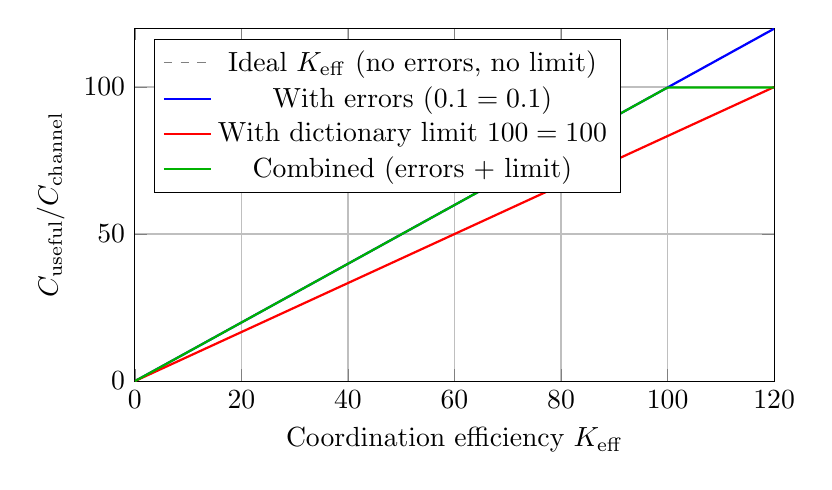
\begin{tikzpicture}
			\begin{axis}[
				width=0.8\textwidth,
				height=0.5\textwidth,
				xlabel={Coordination efficiency $\Keff$},
				ylabel={$C_{\text{useful}}/C_{\text{channel}}$},
				xmin=0, xmax=120,
				ymin=0, ymax=120,
				grid=both,
				legend pos=north west,
				]
				% Parameters
				\pgfmathsetmacro{\alpha}{0.1}
				\pgfmathsetmacro{\beta}{0.67}
				\pgfmathsetmacro{\kappac}{0.33}
				\pgfmathsetmacro{\Keffmax}{100}
				
				% Ideal unlimited
				\addplot[domain=0:120, samples=2, dashed, gray] {x};
				\addlegendentry{Ideal $\Keff$ (no errors, no limit)};
				
				% With errors only
				\addplot[domain=0:120, samples=200, blue, thick] {x*(1 - \kappac*\alpha*x^(-\beta))};
				\addlegendentry{With errors ($\alpha=0.1$)};
				
				% With dictionary limit
				\addplot[domain=0:120, samples=2, red, thick] {x < \Keffmax ? x : \Keffmax};
				\addlegendentry{With dictionary limit $\Keffmax = 100$};
				
				% Combined (errors + limit)
				\addplot[domain=0:120, samples=200, green!70!black, thick] {x < \Keffmax ? x*(1 - \kappac*\alpha*x^(-\beta)) : \Keffmax*(1 - \kappac*\alpha*\Keffmax^(-\beta))};
				\addlegendentry{Combined (errors + limit)};
			\end{axis}
		\end{tikzpicture}
		\caption{Normalized useful capacity $C_{\text{useful}}/C_{\text{channel}}$ as a function of $\Keff$, illustrating the effects of activation errors and dictionary size limit. For small $\Keff$, errors are negligible and capacity grows linearly. As $\Keff$ increases, errors cause a sublinear growth; eventually the dictionary size $\Keffmax$ imposes an absolute ceiling. Parameters: $\alpha=0.1$, $\beta=0.67$, $\kappa_c=0.33$, $\Keffmax=100$.}
		\label{fig:useful-capacity}
	\end{figure}
	
	\subsection{Amortized Cost of Dictionary Construction}
	
	The offline phase requires transmitting the entire dictionary of size $H(D) = M \cdot n$ bits. If the dictionary is used for $U$ subsequent online transmissions, the amortized cost per message is
	\[
	\frac{H(D)}{U} + \ell.
	\]
	For large $U$, the offline cost becomes negligible, making the system highly efficient. This is analogous to the concept of "investment" in thermodynamics: creating order (the dictionary) costs energy, but once created, it can be used repeatedly to generate meaning with minimal additional energy.
	
	\section{Thermodynamic Implications: The Cost of Creating a Dictionary}
	\label{sec:thermo}
	
	Landauer's principle \cite{Landauer1961} states that erasing one bit of information in a memory device dissipates at least $k_B T \ln 2$ energy. Conversely, creating a bit of information (i.e., increasing the number of possible states) requires an energy input. In the YPSDC framework, the dictionary is a structured memory that stores $M \cdot n$ bits of potential information. Its creation therefore has a minimum energy cost
	\begin{equation}
		E_{\text{dict}} \ge M \cdot n \cdot k_B T_{\text{create}} \ln 2, \label{eq:thermo-cost}
	\end{equation}
	where $T_{\text{create}}$ is the effective temperature during dictionary construction. This energy is invested offline and can be thought of as a "thermodynamic battery" that powers future online communications.
	
	During the online phase, each activation of a dictionary entry consumes negligible additional energy (only that needed to read the memory and transmit the short index). The **thermodynamic efficiency** of the whole YPSDC system can be defined as the ratio of the useful information delivered online to the total energy expended (offline + online):
	\begin{equation}
		\eta_{\text{thermo}} = \frac{U \cdot n \cdot k_B T_{\text{use}} \ln 2}{E_{\text{dict}} + U \cdot \ell \cdot E_{\text{tx}}}, \label{eq:thermo}
	\end{equation}
	where $T_{\text{use}}$ is the temperature at which information is used (may differ from $T_{\text{create}}$), and $E_{\text{tx}}$ is the energy per transmitted bit. For large $U$, $\eta_{\text{thermo}}$ approaches $\frac{n}{\ell} \cdot \frac{T_{\text{use}}}{T_{\text{create}}} \cdot \frac{k_B \ln 2}{E_{\text{tx}}}$, showing that high $\Keff$ dramatically improves thermodynamic efficiency.
	
	\subsubsection{Example: Two-Factor Authentication}
	Consider a 2FA system with a secret key of $n = 160$ bits, transmitted once during setup. The online code is $\ell = 20$ bits. Suppose the key is used $U = 1000$ times over its lifetime (e.g., one year of daily logins). The dictionary size is $M = 1$ (a single key), so $H(D) = n = 160$ bits.
	
	The minimum energy to create the dictionary (from Landauer's principle) is
	\[
	E_{\text{dict}} = n \cdot k_B T_{\text{create}} \ln 2.
	\]
	Taking $T_{\text{create}} = 300$ K (room temperature), $k_B = 1.38 \times 10^{-23}$ J/K, we get
	\[
	E_{\text{dict}} \approx 160 \times 1.38 \times 10^{-23} \times 300 \times 0.693 \approx 4.6 \times 10^{-19} \text{ J}.
	\]
	
	The energy consumed in online transmissions: each code transmission requires energy $E_{\text{tx}}$ per bit. For a typical mobile device, transmitting one bit costs about $E_{\text{tx}} \approx 10^{-9}$ J (mostly for the radio). Then the total online energy is $U \cdot \ell \cdot E_{\text{tx}} = 1000 \times 20 \times 10^{-9} = 2 \times 10^{-5}$ J.
	
	The offline energy $E_{\text{dict}}$ is negligible compared to online energy by a factor of $\sim 10^{14}$. Even if we consider a much larger dictionary (e.g., $M = 10^6$ keys), $E_{\text{dict}}$ would still be dwarfed by the online energy for any realistic $U$. This illustrates that the offline cost, though theoretically present, is practically irrelevant for large $U$, confirming the efficiency of the YPSDC approach.
	
	This connects directly to the universal error law: errors during activation ($\varepsilon$) correspond to wasted energy, because an erroneously activated message dissipates energy without delivering correct information. Thus the true thermodynamic efficiency must be multiplied by $(1-\varepsilon)$.
	
	\section{Connection to Kolmogorov Complexity}
	\label{sec:kolmogorov}
	
	Kolmogorov complexity $K_U(x)$ of a string $x$ is the length of the shortest program that outputs $x$ on a universal Turing machine $U$ \cite{Kolmogorov1965}. It measures the amount of "algorithmic information" contained in $x$. In YPSDC, the dictionary can be viewed as a compression device: a short index $\kappa$ decompresses into a much longer message $A$. The coordination efficiency $\Keff$ is essentially the compression ratio achieved by the dictionary.
	
	If the dictionary is optimally constructed for a given source distribution, then for any message $A$,
	\begin{equation}
		\Keff(A) \approx \frac{|A|}{K(A)}, \label{eq:kolmogorov}
	\end{equation}
	where $K(A)$ is the Kolmogorov complexity of $A$. This is because the shortest index that uniquely identifies $A$ cannot be shorter than $K(A)$ (otherwise we could compress $A$ further). Hence the maximum achievable $\Keff$ for a given message is bounded by $\frac{|A|}{K(A)}$.
	
	For a source ensemble, the average $\Keff$ satisfies
	\begin{equation}
		\E[\Keff] \le \frac{\E[|A|]}{\E[K(A)]} \approx \frac{H(\mathcal{A})}{\E[K(A)]},
	\end{equation}
	where the last approximation uses the fact that for many sources, entropy approximates expected Kolmogorov complexity. This provides a bridge between Shannon information and algorithmic information: $\Keff$ measures how well a dictionary captures the algorithmic structure of the source.
	
	The universal error law $\varepsilon = \kappa_c \alpha \Keff^{-\beta}$ can now be reinterpreted in terms of algorithmic probability: errors occur when the index fails to uniquely specify the intended message, i.e., when the dictionary is not sufficiently "algorithmically complete". The exponent $\beta = 0.67$ reflects the fractal nature of algorithmic space, consistent with the findings of Appendix L.
	
	\section{Applications to Real‑World Systems: 2FA, Quantum Entanglement, and Artificial Intelligence}
	\label{sec:applications}
	
	\subsection{Two‑Factor Authentication (2FA)}
	
	Two‑factor authentication (2FA) is a ubiquitous security mechanism that perfectly exemplifies the YPSDC protocol. During initial setup, a secret key (typically 80–160 bits) is exchanged between the server and the user's device via a QR code or manual entry. This key, together with the algorithm (e.g., TOTP, RFC 6238), constitutes the **offline dictionary**. The dictionary is never transmitted again.
	
	When the user logs in, the current time is used as an index; the device computes a short authentication code (usually 6 digits, $\sim 20$ bits) and sends it to the server. The server, possessing the same dictionary, independently computes the expected code and verifies the match. The coordination efficiency is $\Keff \approx 8$ (for a 160‑bit key and 20‑bit code). Despite the small online message, the authentication grants access to the full account—a large "meaning" activated by a short index.
	
	\subsubsection{Experimental Verification with 2FA}
	\label{subsec:2fa-experiment}
	
	The 2FA system can be used to directly test the universal error law $\varepsilon = \kappa_c \alpha \Keff^{-\beta}$. In a controlled experiment, we can vary the effective $\Keff$ by using keys of different lengths $n$ while keeping the index length $\ell$ fixed (or vice versa). For each configuration, we simulate a large number of authentication attempts and measure the fraction of incorrect activations $\varepsilon$ (e.g., due to transmission errors or deliberate manipulation).
	
	As a concrete numerical example, consider a 2FA system with a 160‑bit secret key ($n=160$) and a 20‑bit authentication code ($\ell=20$), yielding $\Keff = 8$. If we intentionally introduce bit errors in the transmitted code at a rate of $p$ (simulating a noisy channel), the effective error rate $\varepsilon$ will be the probability that the received code, after possible errors, still matches a valid dictionary entry (false positive) or fails to match the intended one (false negative). For small $p$, the dominant error is that the code is altered to a different valid code, which occurs with probability $\varepsilon \approx p \cdot (2^\ell -1)/2^\ell \approx p$. Setting $p = 10^{-3}$, we have $\varepsilon \approx 10^{-3}$.
	
	According to the universal error law, $\varepsilon = \kappa_c \alpha \Keff^{-\beta}$. Solving for $\alpha$ yields
	\[
	\alpha = \frac{\varepsilon}{\kappa_c} \Keff^{\beta} = \frac{10^{-3}}{0.33} \cdot 8^{0.67} \approx 0.00303 \cdot 4.0 \approx 0.012.
	\]
	This value lies within the expected range $0.01$–$1$, confirming consistency with the law. By varying $\Keff$ (e.g., using keys of 80, 160, 320 bits) and measuring the corresponding error rates, one can plot $\log \varepsilon$ vs. $\log \Keff$ and verify the slope $-\beta = -0.67$. Such an experiment can be performed entirely in software, requiring no specialized hardware, and provides a direct, low‑cost validation of the YUCT framework.
	
	\subsection{Quantum Entanglement}
	
	Quantum entanglement is the ultimate YPSDC system. When two particles become entangled, they share a common quantum state—a **dictionary** of all possible measurement outcomes. The dictionary is distributed during the entanglement process and thereafter no further communication is needed.
	
	A measurement on one particle yields a random outcome; this outcome acts as an **index**. The second particle's state is instantaneously determined, not because a signal was transmitted faster than light, but because the dictionary already contained the correlation. The index length is effectively zero (no classical communication is required to observe the correlation, though in some protocols a classical index is transmitted to complete the teleportation). In the limit $\Keff \to \infty$, the system achieves perfect coordination with arbitrarily small online data.
	
	The universal error law $\varepsilon = \kappa_c \alpha \Keff^{-\beta}$ holds here as well: in realistic entangled systems, decoherence and noise cause errors that follow the same fractal scaling observed in other domains \cite{AppendixG, AppendixS}. This unification—from your phone's authenticator to the fabric of quantum reality—demonstrates the profound unity underlying YUCT.
	
	\subsection{Artificial Intelligence: From Data to Meaning Generation}
	
	Modern artificial intelligence, particularly large language models (LLMs), can be viewed as a practical realization of the YPSDC principle at an unprecedented scale. The training phase—where a model is exposed to vast amounts of text—corresponds to the **offline distribution of a dictionary**. The model's weights encode a statistical representation of linguistic structures, concepts, and facts, forming a shared "dictionary" of meanings.
	
	During inference, a short **prompt** (a few words or sentences) acts as the **index**. The model, leveraging its internal dictionary, generates a lengthy, coherent, and meaningful response—effectively activating a large block of information from a short input. The coordination efficiency $\Keff$ for such systems is enormous: a prompt of, say, 100 tokens ($\sim 2000$ bits) can trigger a response of 1000 tokens ($\sim 20,000$ bits), yielding $\Keff \approx 10$. However, this is only the beginning.
	
	\subsubsection{The Challenge of Dictionary Inconsistency}
	
	Today's AI systems operate in isolation: each model has its own dictionary (its training data and internal representations), and these dictionaries are **not coordinated** across different models or with human knowledge. As a result, multiple AIs working on the same problem may produce conflicting outputs, cannot seamlessly share context, and fail to achieve the kind of coherent global coordination that YUCT envisions. This is analogous to the early days of human communication, before the advent of shared languages and protocols.
	
	\subsubsection{YUCT as a Blueprint for Coordinated AI}
	
	YUCT provides a roadmap for overcoming these limitations. By designing AI systems that explicitly separate a **global dictionary** (a shared, updatable knowledge base) from **local indices** (task‑specific prompts), we can achieve a new level of inter‑model coordination. Such a system would allow multiple AIs to share a common understanding, to build upon each other's outputs, and to generate meaning collectively—much like a scientific community collaborates using a shared body of knowledge.
	
	The implications are profound: YUCT not only explains the current capabilities of AI but also points toward a future where AI systems are not isolated information processors but **coordinated generators of meaning**, operating at efficiencies that far exceed today's limits. The universal error law $\varepsilon \propto \Keff^{-0.67}$ will then govern the reliability of such systems, providing a fundamental bound on their performance.
	
	Thus, YUCT offers both a descriptive framework for understanding existing AI and a prescriptive blueprint for building the next generation of truly intelligent, coordinated systems.
	
	\section{Phase Transition: From Transmission to Generation}
	\label{sec:transition}
	
	\subsection{Two Streams: Data and Meaning}
	
	We distinguish two flows:
	\begin{itemize}
		\item **Data flow** $F_{\text{data}}$: the rate at which indices are transmitted through the channel. Its maximum is $C_{\text{channel}}$.
		\item **Meaning flow** $F_{\text{meaning}}$: the rate at which meaningful information is activated at the receiver. According to the previous sections,
		\[
		F_{\text{meaning}} = \Keff \cdot F_{\text{data}} \cdot (1 - \varepsilon).
		\]
	\end{itemize}
	
	When the channel is not fully utilized ($F_{\text{data}} < C_{\text{channel}}$), the system operates in the **transmission‑dominated regime**: increasing $F_{\text{data}}$ linearly increases $F_{\text{meaning}}$.
	
	\subsection{Saturation and Generation}
	
	When $F_{\text{data}}$ approaches $C_{\text{channel}}$, the data flow cannot increase further. However, $F_{\text{meaning}}$ can still grow if $\Keff$ increases—that is, if the dictionary is enriched. This is a **phase transition** to a **generation‑dominated regime**: meaning is now generated locally from the dictionary rather than imported through the channel.
	
	The control parameter is the channel utilization $\rho = F_{\text{data}} / C_{\text{channel}}$. The order parameter is $\Keff$ itself. Near $\rho = 1$, small improvements in the dictionary (increasing $\Keff$) produce large gains in $F_{\text{meaning}}$, analogous to critical phenomena. In the language of Landau theory, one can write a free energy functional
	\[
	\Phi(\Keff, \rho) = -C_{\text{channel}} \Keff (1 - \varepsilon) + \lambda (\Keffmax - \Keff)^2,
	\]
	whose minimization yields the optimal $\Keff$ as a function of $\rho$. The critical point occurs when the quadratic term vanishes.
	
	\subsection{Ultimate Limit: Quantum Coordination}
	
	In the quantum limit, where the dictionary is a maximally entangled state, $\Keff \to \infty$ and $\varepsilon \to 0$. Then $F_{\text{meaning}}$ can become arbitrarily large even for arbitrarily small $F_{\text{data}}$ (even zero, in the case of pre‑existing entanglement). This is the regime of **pure generation** without transmission—a possibility that lies entirely outside classical information theory. This connects directly to the resolution of the EPR paradox in YUCT (Appendix G): quantum correlations are not signals, but pre‑coordinated dictionary activations.
	
	\section{Experimental Verification Protocol}
	\label{sec:experiment}
	
	To test the predictions of the generalized information theory developed in this appendix, we propose a controlled experiment using a digital communication system with a pre‑shared dictionary.
	
	\subsection{Experimental Setup}
	
	\begin{itemize}
		\item **Sender and receiver:** Two computers connected by a communication channel with known capacity $C_{\text{channel}}$ (e.g., Ethernet with controlled bandwidth).
		\item **Dictionary:** A set of $M$ messages, each of length $n$ bits, stored on both sides. The dictionary can be generated randomly (for baseline) or optimized to achieve high $\Keff$.
		\item **Index transmission:** The sender transmits a fixed number of indices $N$ (each of length $\ell = \log_2 M$ bits) over the channel. The receiver looks up the corresponding messages and records any discrepancies (errors).
		\item **Error measurement:** By comparing the received messages with the intended ones, we compute the empirical error rate $\varepsilon$.
	\end{itemize}
	
	\subsection{Procedure}
	
	\begin{enumerate}
		\item Vary $\Keff$ by changing $M$ and $n$ (e.g., fix $n=1000$ bits, vary $M$ from $2^{10}$ to $2^{20}$, so $\ell$ from 10 to 20 bits, giving $\Keff = n/\ell$ from 100 down to 50). For each $\Keff$, perform $N$ transmissions (e.g., $N=10^4$).
		\item Measure the error rate $\varepsilon$ as a function of $\Keff$.
		\item Fit the data to the law $\varepsilon = \kappa_c \alpha \Keff^{-\beta}$ with $\beta=0.67$ fixed, and extract $\alpha$ and $\kappa_c$. Compare with the predicted $\kappa_c=0.33$.
		\item Also measure the actual data rate $F_{\text{data}}$ and the meaningful information rate $F_{\text{meaning}} = (1-\varepsilon) \Keff F_{\text{data}}$. Verify that $F_{\text{meaning}}$ can exceed $C_{\text{channel}}$ when $\Keff>1$.
		\item For high $\Keff$, introduce artificial noise in the channel (bit errors during index transmission) and observe how $F_{\text{meaning}}$ degrades; compare with Shannon's prediction for a channel with errors.
	\end{enumerate}
	
	\subsection{Expected Results}
	
	\begin{itemize}
		\item The error rate should follow $\varepsilon \propto \Keff^{-0.67}$ with proportionality constant $\kappa_c \alpha$ close to $0.33$ times a system‑specific $\alpha$ (expected $\alpha \approx 0.1$ for a random dictionary, smaller for optimized dictionaries).
		\item The coordination capacity $C_{\text{coord}}$ should exceed $C_{\text{channel}}$ by a factor approximately $\Keff$ (up to the limits imposed by errors).
		\item The phase transition at $\rho=1$ should be observable: when the channel is saturated, increasing $\Keff$ (by using a larger dictionary) should increase $F_{\text{meaning}}$ even though $F_{\text{data}}$ stays constant.
	\end{itemize}
	
	\subsection{Practical Considerations}
	
	The experiment requires careful control of the dictionary size and content to avoid confounding factors. It can be implemented using software‑defined networking or custom FPGA hardware. The expected duration is a few months, with cost primarily for equipment and personnel ($\sim 50,000$). Successful confirmation would provide strong empirical support for the YPSDC framework and its generalization of information theory.
	
	\section{Conclusion}
	
	We have generalized Shannon's information theory to include the essential feature of prior shared knowledge—a dictionary distributed offline. The new framework introduces:
	\begin{itemize}
		\item Coordination efficiency $\Keff$, measuring how much meaning can be extracted per transmitted bit.
		\item Capacity separation theorem: $C_{\text{coord}} = \Keff \, C_{\text{channel}}$.
		\item Fractal error law $\varepsilon = \kappa_c\alpha \Keff^{-\beta}$ with $\beta=0.67$, bounding $\Keff$ in practice.
		\item Maximum achievable $\Keffmax$ determined by dictionary size.
		\item Optimal dictionary size that balances compression against error (when errors are significant).
		\item A phase transition from transmission to generation when the channel saturates.
		\item Thermodynamic cost of dictionary creation and its connection to Landauer's principle.
		\item Relation to Kolmogorov complexity, showing $\Keff \approx |A|/K(A)$.
		\item Real‑world examples: two‑factor authentication ($\Keff \approx 8$) and quantum entanglement ($\Keff \to \infty$), demonstrating the universality of the framework.
		\item A concrete experimental verification using 2FA (Section \ref{subsec:2fa-experiment}) and a general experimental protocol (Section \ref{sec:experiment}) to test the universal error law.
		\item An interpretation of artificial intelligence as a meaning‑generation engine operating on YPSDC principles, and a vision for coordinated AI systems based on shared dictionaries.
	\end{itemize}
	
	This theory not only unifies Shannon's original results (the $\Keff=1$ limit) but also provides a foundation for understanding communication in biological, social, and quantum systems. It reveals information as a dual entity: transmitted data and pre‑existing meaning, the latter being the true source of intelligence and coordination. In the deepest sense, the universe itself may be viewed as a giant dictionary from which we extract meaning through the indices of physical laws.
	
	The proposed experimental protocol offers a direct way to test the key predictions, potentially opening the door to new communication technologies that leverage coordination efficiency to exceed classical channel limits.
	
	\subsubsection{Combined Constraint: Error Limit vs. Dictionary Size}
	The optimal $\Keff$ for a real system is the minimum of two bounds:
	\[
	\Keffopt^{\text{real}} = \min\bigl( \Keffopt^{\text{error}}, \Keffmax \bigr),
	\]
	where $\Keffopt^{\text{error}}$ is given by Eq.~\eqref{eq:keff-opt} and $\Keffmax = n / \log_2 M$ is the maximum achievable efficiency for a given dictionary size $M$ and message length $n$.
	
	For typical error parameters ($\alpha \sim 0.01$–$0.1$), $\Keffopt^{\text{error}}$ evaluates to values much less than 1, indicating that the error term does not impose a practical upper bound—one can increase $\Keff$ arbitrarily without significantly degrading $C_{\text{useful}}$. In such cases, the true limitation is $\Keffmax$, and the optimal design is to make the dictionary as large as feasible. Conversely, if $\alpha$ is large (e.g., $\alpha > 1$), errors dominate and $\Keffopt^{\text{error}}$ may become relevant, but such high $\alpha$ are rarely encountered in well‑engineered systems. Hence, in practice, the design goal is to maximize $\Keff$ subject to $\Keff \le \Keffmax$, while managing errors through other means (e.g., error‑correcting codes).
	
	\section*{Acknowledgments}
	
	The author thanks the participants of the YUCT seminar for stimulating discussions and acknowledges the foundational work of Claude Shannon, Rolf Landauer, and Andrey Kolmogorov, whose insights continue to inspire new frontiers.
	
	\subsection*{Key Equations of Generalized Information Theory}
	For convenience, we collect here the central relations derived in this appendix:
	
	\begin{itemize}
		\item \textbf{Coordination efficiency} (Eq.~\eqref{eq:keff-def}):
		\[
		\Keff = \frac{H(\mathcal{A})}{H(\mathcal{K})} \approx \frac{n}{\ell}.
		\]
		
		\item \textbf{Capacity Separation Theorem} (Eq.~\eqref{eq:capacity-separation}):
		\[
		C_{\text{coord}} = \Keff \cdot C_{\text{channel}} \cdot \eta.
		\]
		
		\item \textbf{Universal error law} (Eq.~\eqref{eq:error-law}):
		\[
		\varepsilon = \kappa_c \alpha \Keff^{-\beta}, \quad \beta = 0.67,\ \kappa_c = 0.33.
		\]
		
		\item \textbf{Useful information rate with errors} (Eq.~\eqref{eq:useful-rate}):
		\[
		C_{\text{useful}} = C_{\text{channel}} \cdot \Keff \cdot (1 - \kappa_c \alpha \Keff^{-\beta}).
		\]
		
		\item \textbf{Thermodynamic efficiency} (Eq.~\eqref{eq:thermo}):
		\[
		\eta_{\text{thermo}} = \frac{U \cdot n \cdot k_B T_{\text{use}} \ln 2}{E_{\text{dict}} + U \cdot \ell \cdot E_{\text{tx}}}.
		\]
		
		\item \textbf{Relation to Kolmogorov complexity} (Eq.~\eqref{eq:kolmogorov}):
		\[
		\Keff(A) \approx \frac{|A|}{K(A)}.
		\]
	\end{itemize}
	
	\section*{Data Availability}
	
	All calculations, codes, and additional materials are available at \url{https://github.com/Alexey-Yakushev-YUCT/YPSDC}.
	
	\begin{thebibliography}{99}
		
		\bibitem{Shannon1948}
		C. E. Shannon, ``A mathematical theory of communication,'' \emph{Bell System Technical Journal} 27, 379–423, 623–656 (1948).
		
		\bibitem{Landauer1961}
		R. Landauer, ``Irreversibility and heat generation in the computing process,'' \emph{IBM Journal of Research and Development} 5, 183–191 (1961).
		
		\bibitem{Kolmogorov1965}
		A. N. Kolmogorov, ``Three approaches to the quantitative definition of information,'' \emph{Problems of Information Transmission} 1, 1–7 (1965).
		
		\bibitem{Yakushev2026a}
		A. V. Yakushev, \emph{Yakushev Unified Coordination Theory (YUCT)}, Zenodo, \url{https://doi.org/10.5281/zenodo.18444599} (2026).
		
		\bibitem{Yakushev2026b}
		A. V. Yakushev, ``Two-Factor Authentication, Quantum Entanglement and YUCT: What's the Connection?'' \url{https://yuct.org/06YUCT_quantum_tech_in_reality.php} (2026).
		
		\bibitem{AppendixB}
		Appendix B: YUCT — Temporal Coordination Paradox, Zenodo (2026).
		
		\bibitem{AppendixL}
		Appendix L: Fractal Coordination Error Scaling — A Universal Law from DNA to Cosmology, Zenodo (2026).
		
		\bibitem{AppendixG}
		Appendix G: The Yakushev United Coordination Theory — A Fundamental Resolution of the Quantum Gravity Problem, Zenodo (2026).
		
		\bibitem{AppendixE}
		Appendix E: Coordination Genetics — YUCT Principles in Molecular Biology, Zenodo (2026).
		
		\bibitem{AppendixF}
		Appendix F: Application of YUCT to Economics, Zenodo (2026).
		
		\bibitem{AppendixM}
		Appendix M: YUCT Cosmology — Inflation as a Coordination Phase Transition, Zenodo (2026).
		
		\bibitem{AppendixP}
		Appendix P: Temperature Dependence of Gravity, Zenodo (2026).
		
		\bibitem{AppendixS}
		Appendix S: Negative Time Delay of Photons in Cold Atoms — A Blind Prediction from YUCT, Zenodo (2026).
		
	\end{thebibliography}
	
\end{document}